\chapter{Аналитическая часть}

В данном разделе рассмотрены теоретические выкладки по алгоритмам сортировки. В дальнейшем в рамках данной работы предполагается, что происходит сортировка набора целых чисел по возрастанию.

\section{Блочная сортировка}
Блочная сортировка~---~алгоритм сортировки, в котором происходит разбиение входного набора элементов на блоки, причем значения элементов в каждом блоке больше, чем в предыдущем.
После разбиения входного набора элементов на блоки, происходит сортировка каждого блока по отдельности, либо рекурсивно с использованием блочной сортировки, либо с использованием другого алгоритма сортировки.
После сортировки блоков, так как значения в каждом блоке больше, чем в предыдущем, происходит слияние блоков, в результате которого получается отсортированный набор.

Пример разбиения на блоке представлен на рис. \ref{img:block_example}.

\begin{figure}[h!]
\centering
    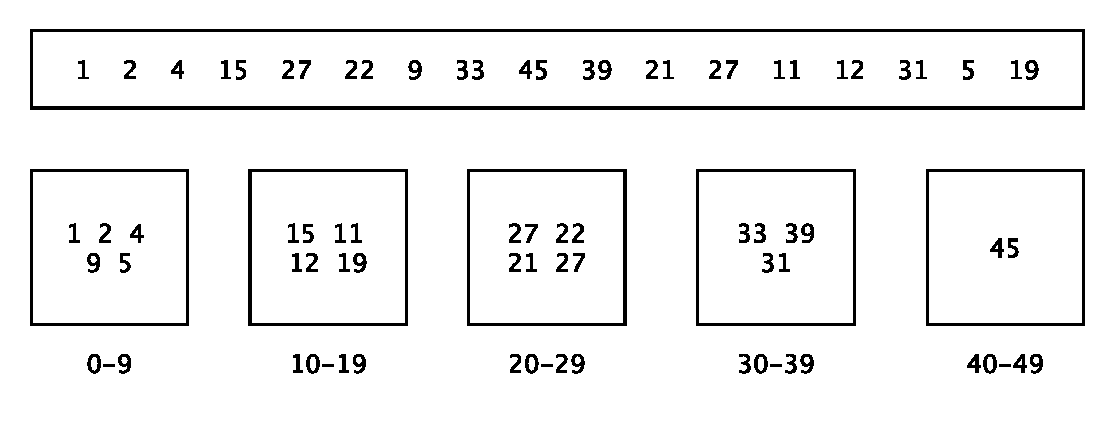
\includegraphics[width=0.6\linewidth]{block_example.pdf}
    \caption{Пример разбиения входного набора чисел на блоки}
    \label{img:block_example}	
\end{figure}


\section{Пирамидальная сортировка}
Пирамидальная сортировка~---~алгоритм сортировки, в котором на заданном массиве происходит создание такой структуры данных, как пирамида \cite{bib:heapsort_info}. 
Пирамида определяется как последовательность элементов $a_{l}, a_{l+1}, \ldots, a_{r}$ такая, что 

\begin{equation}
	\forall i = l \ldots \frac{r}{2}: \begin{cases}
		a_{i} \le a_{2 \cdot i}, \\
		a_{i} \le a_{2 \cdot i + 1}.
	\end{cases}
\end{equation}

Если представлять пирамиду как древовидную структуру, то в корневой вершине дерева будет находиться минимальный элемент. 
Соответственно, если построить такую структуру на входном наборе данных, то минимальный элемент встанет на свою позицию, так как в результате построения пирамиды, минимальный элемент будет найден.
 Для дальнейшей сортировки требуется рассмотреть пирамидальную структуру на оставшемся наборе данных.


\section{Сортировка подсчетом}
Сортировка подсчетом~---~алгоритм сортировки, в котором происходит подсчет количества вхождений каждого элемента в исходный набор данных. 
На основе собранной статистики, происходит создание отсортированного массива. 
Особенностью данного алгоритма является то, что он работает только с наборами целых чисел.

\newpage